%%%%%%%%%%%%%%%%%%%%%%%%%%%%%%%%%%%%%%%%%%%%%%%%%%%%%%%%%%%%%%%%%%%%%%%%%%%%%%%
\section{Programming interfaces}
%%%%%%%%%%%%%%%%%%%%%%%%%%%%%%%%%%%%%%%%%%%%%%%%%%%%%%%%%%%%%%%%%%%%%%%%%%%%%%%
%------------------------------------------------------------------------------
%%%%%%%%%%%%%%%%%%%%%%%%%%%%%%%%%%%%%%%%%%%%%%%%%%%%%%%%%%%%%%%%%%%%%%%%%%%%%%%
\subsection{OmpSs}
%------------------------------------------------------------------------------
\begin{frame}
  \frametitle{OmpSs}
  \begin{itemize}
  \item Task-based data flow programming model with single address space.
  \item Target platforms:
    \begin{itemize}
    \item multicore / SMP machines.
    \item heterogeneous systems (GPUs, Cell BE).
    \item clusters / distributed systems.
    \end{itemize}
  \item Based on OpenMP \blue{pragmas}.
    \begin{itemize}
    \item OpenMP + StarSs extensions.
    \end{itemize}
  \end{itemize}
  %
  \begin{block}{Data dependency}
    \begin{itemize}
    \item {\bf in} - read-only.
    \item {\bf out} - write-only.
    \item {\bf inout} - read and write.
    \item {\bf concurrent} - cumulative write.
    \end{itemize}
  \end{block}
\end{frame}
%------------------------------------------------------------------------------
\begin{frame}[fragile]
  \frametitle{OmpSs}
  %
  \begin{itemize}
  \item Task dependencies based on OpenMP.
  \end{itemize}
  %
  \begin{block}{}
\begin{lstlisting}
int main(void)
{
#pragma omp task out(result1)
  result1 = compute();

#pragma omp task in(result1)
  print(result1);

#pragma omp taskwait

  return 0;
}
\end{lstlisting}
  \end{block}
\end{frame}
%------------------------------------------------------------------------------
\begin{frame}[fragile]
  \frametitle{OmpSs}
  \begin{block}{}
\begin{lstlisting}
int reduce( int *a, int n ) {
  int i, result = 0;
  for(i= 0; i < n; i++){
#pragma omp task concurrent(result)
#pragma omp atomic
    result += a[i];
  }
  return result;
}

int main(void)
{
  int a[100];

#pragma omp task out(a)
  generate(a, 100);
  reduce(a, 100);

  return 0;
}
\end{lstlisting}
  \end{block}
\end{frame}
%------------------------------------------------------------------------------
\begin{frame}[fragile]
  \frametitle{Blocked matrix multiplication}
  \begin{block}{}
\begin{lstlisting}
#pragma omp target device (smp) 
#pragma omp task in([BS*BS]A, [BS*BS]B) inout([BS*BS]C)
void matmul_tile(float *A, float *B, float *C, int BS) {
  cblas_dgemm(CblasRowMajor, CblasNoTrans, CblasNoTrans,
       BS, BS, BS, 1.0, A, BS, B, BS, 1.0, C, BS);
}

void matmul(int mb, int nb, int kb,
                          float **A, float **B, float **C, int BS) { 
  int i, j, k;
  for(i = 0; i < mb; i++)
      for(j = 0; j < nb; j++)
        for(k = 0; k < kb; k++)
          matmul_tile(A[i*mb+k], B[k*kb+j], C[i*mb+j], BS);
}
\end{lstlisting}
\end{block}
\end{frame}
%------------------------------------------------------------------------------
\begin{frame}[fragile]
  \frametitle{OmpSs and GPUs}
  \begin{block}{}
\begin{lstlisting}
#pragma omp target device (smp) copy_deps
#pragma omp task 
void compute(void) {
    /* CPU */
}

#pragma omp target device (cuda) implements(compute) copy_deps
#pragma omp task 
void compute_cuda(void) {
    /* CUDA */
}

int main(void)
{
  compute();

  return 0;
}
\end{lstlisting}
  \end{block}
%
\pause
%
  \begin{alertblock}{Notice}
    In this tutorial, we do not detail heterogeneous systems.
  \end{alertblock}
\end{frame}
%------------------------------------------------------------------------------
\begin{frame}[fragile]
  \frametitle{Scheduling policy}
  \begin{itemize}
  \item {\bf breadth first} (\texttt{bf}) - global queue with tasks in FIFO.
  \item {\bf distributed breadth first} (\texttt{dbf}) - one queue per thread, with 
      task stealing.
  \item {\bf work first} (\texttt{wf}) - same of \texttt{dbf}, but it executes a 
    newly created task (depth-first).
  \item {\bf socket-aware} (\texttt{socket}) - per-socket level queue, it may use work stealing.
  \item {\bf versioning} (\texttt{versioning}) - multiple task implementations, using the 
    most suitable for the target.
  \end{itemize}
  %
  \begin{exampleblock}{Selecting a policy}
  \verb+$ NX_SCHEDULE=wf ./program+
  \end{exampleblock}
\end{frame}
%------------------------------------------------------------------------------
\begin{frame}[fragile]
  \frametitle{Installing OmpSs}
  \begin{itemize}
  \item Two step installation: \blue{Nanos++} and \blue{Mercurium C/++}.
    \begin{itemize}
    \item \blue{Nanos++}: runtime system.
    \item \blue{Mercurium C/C++ compiler}: compiler system (source-to-source).
    \end{itemize}
  \item Target \verb+export TARGET=$HOME/ompss+.
  \end{itemize}
  %
  \begin{block}{}
\begin{lstlisting}[language=]
$ cd ompss-yy.mm/nanox-version
$ ./configure --prefix=$TARGET
$ make
$ make install
\end{lstlisting}
  \end{block}
  %
  \begin{block}{}
\begin{lstlisting}[language=]
$ cd ompss-yy.mm/mcxx-version
$ ./configure --prefix=$TARGET --enable-ompss --with-nanox=$TARGET
$ make
$ make install
\end{lstlisting}
  \end{block}
  %
  \begin{alertblock}{Website}
    \begin{center}
      \url{https://pm.bsc.es/ompss}
    \end{center}
  \end{alertblock}
\end{frame}
%------------------------------------------------------------------------------
%%%%%%%%%%%%%%%%%%%%%%%%%%%%%%%%%%%%%%%%%%%%%%%%%%%%%%%%%%%%%%%%%%%%%%%%%%%%%%%
\subsection{StarPU}
%------------------------------------------------------------------------------
\begin{frame}
  \frametitle{StarPU}
  \begin{itemize}
  \item Runtime system for heterogeneous architectures.
    \begin{itemize}
    \item multi-CPUs, multi-GPUs, Cell BE.
    \end{itemize}

  \item Task-based programming model with data dependencies.

  \item Three main concepts:
    \begin{itemize}
    \item {\bf Codelet}  - describes a computational kernel.
    \item {\bf Task} - instance of a codelet.
    \item {\bf Data handle} - data entity that keeps track of copies over memory nodes.
    \end{itemize}
  \end{itemize}
\end{frame}
%------------------------------------------------------------------------------
%\begin{frame}[fragile]
%  \frametitle{StarPU vector scaling}
%  %
%  \begin{itemize}
%  \item First, select the \blue{performance model}.
%    \begin{itemize}
%    \item<2-> model type.
%    \item<3-> name of the 
%    \end{itemize}
%  \end{itemize}
%  %
%  \begin{block}{}
%\begin{lstlisting}[name=starpuvector,firstnumber=auto]
%/* Here it selects the history-based performance model */
%static struct starpu_perfmodel vector_scal_model = {
%  .type = STARPU_HISTORY_BASED,	
%  .symbol = "vector_scale_model"
%};
%
%\end{lstlisting}
%  \end{block}
%\end{frame}
%------------------------------------------------------------------------------
\begin{frame}[plain,fragile]
  \frametitle{StarPU vector scaling}
  %
  \begin{itemize}
  \item StarPU main program:
    \begin{itemize}
    \item<2-> Initialize StarPU with default configuration.
    \item<3-> Call the compute function.
    \item<4-> Terminate StarPU.
    \end{itemize}
  \end{itemize}
  %
  \begin{block}{}
\begin{lstlisting}[escapeinside={@}{@}]
int main(int argc, char **argv)
{
    float vector[NX];
    float factor = 3.14;
    
    @\alert<2>{starpu\_init(NULL);}@

    @\alert<3>{compute( vector, NX, factor );}@

    @\alert<4>{starpu\_shutdown();}@
    
    return 0;
}
\end{lstlisting}
  \end{block}
\end{frame}
%------------------------------------------------------------------------------
\begin{frame}[fragile]
  \frametitle{StarPU vector scaling}
  %
  \begin{itemize}
  \item Declaring a {\bf codelet}:
    \begin{itemize}
    \item<2-> Plug the kernel function.
    \item<3-> Declare the number of parameters used by the kernel.
    \item<4-> Declare the access mode of each parameter.
    \end{itemize}
  \end{itemize}
  %
  \begin{block}{}
\begin{lstlisting}[escapeinside={@}{@},name=starpuvector,firstnumber=auto]
static struct starpu_codelet cl = {
    @\alert<2>{.cpu\_funcs = \{vector\_scal\_cpu, NULL\},}@
    @\alert<3>{.nbuffers = 1,}@
    @\alert<4>{.modes = \{STARPU\_RW\}}@
};
\end{lstlisting}
  \end{block}
\end{frame}
%------------------------------------------------------------------------------
\begin{frame}[fragile]
  \frametitle{StarPU vector scaling}
  %
  \begin{itemize}
  \item Submitting a task:
    \begin{itemize}
    \item<2-> Tell StarPU to associate ``vector'' with a ``vector\_handle''.
    \item<3-> Insert a task in the StarPU DAG.
    \item<4-> Wait for tasks to complete.
    \item<5-> Stop data monitoring.
    \end{itemize}
  \end{itemize}
  %
  \begin{block}{}
\begin{lstlisting}[escapeinside={@}{@}]
void compute(float* vector, float factor, int n)
{
    @\alert<2>{starpu\_data\_handle\_t vector\_handle;}@
    @\alert<2>{starpu\_vector\_data\_register(\&vector\_handle, 0, (uintptr\_t)vector,}@
                                @\alert<2>{n, sizeof(vector[0]));}@

    @\alert<3>{ret = starpu\_insert\_task( \&cl,}@
                 @\alert<3>{STARPU\_VALUE, \&factor, sizeof(factor),}@
                 @\alert<3>{STARPU\_RW, vector\_handle,}@
                 @\alert<3>{0);}@

    @\alert<4>{starpu\_task\_wait\_for\_all();}@
    @\alert<5>{starpu\_data\_unregister(vector\_handle);}@
}
\end{lstlisting}
  \end{block}
\end{frame}
%------------------------------------------------------------------------------
\begin{frame}[plain,fragile]
  \frametitle{StarPU vector scaling}
  \begin{itemize}
  \item Writing the {\bf kernel function} for CPU:
    \begin{itemize}
    \item<2-> Extract the argument's value.
    \item<3-> Handle and length of the vector.
    \item<4-> Get a pointer to the local copy of the vector.
    \item<5-> Scale the vector.
    \end{itemize}
  \end{itemize}
  %
  \begin{block}{}
\begin{lstlisting}[escapeinside={@}{@}]
void vector_scal_cpu(void *buffers[], void *cl_arg)
{
  unsigned i;
  float factor;

  @\alert<2>{starpu\_codelet\_unpack\_args(cl\_arg, \&factor);}@
  @\alert<3>{struct starpu\_vector\_interface *vector = buffers[0];}@
  @\alert<3>{unsigned n = STARPU\_VECTOR\_GET\_NX(vector);}@
  @\alert<4>{float *val = (float *)STARPU\_VECTOR\_GET\_PTR(vector);}@
  @\alert<5>{for (i = 0; i < n; i++)}@
     @\alert<5>{val[i] *= factor;}@
}
\end{lstlisting}
  \end{block}
\end{frame}
%------------------------------------------------------------------------------
\begin{frame}[fragile]
  \frametitle{Data access mode}
  \begin{itemize}
  \item \textbf{STARPU\_R} - read-only mode.
  \item \textbf{STARPU\_W} - write-only mode.
  \item \textbf{STARPU\_RW} -  read and write mode.
  \item \textbf{STARPU\_SCRATCH} - temporary buffer, with no dependency constraint.
  \item \textbf{STARPU\_REDUX} - cumulative write with reduction.
  \end{itemize}
\end{frame}
%------------------------------------------------------------------------------
\begin{frame}[fragile]
  \frametitle{Performance model}
  \begin{itemize}
  \item Some scheduling policies estimate execution time in advance.
    \begin{itemize}
    \item Ex.: dm, dmda, heft.
    \end{itemize}
  
  \item Codelets give the \blue{performance model} specifying:
    \begin{itemize}
    \item Model name.
    \item Model type.
    \end{itemize}

  \item Available performance models:
    \begin{itemize}
    \item \textbf{STARPU\_HISTORY\_BASED} - measured at runtime. Records the
    average time for each input/output sizes.
    \item \textbf{STARPU\_REGRESSION\_BASED} - linear regression model over different data sizes
       ($\alpha*n^\beta$).
    \item \textbf{STARPU\_NL\_REGRESSION\_BASED} - non-linear regression model ($\alpha*n^\beta+\gamma$).
    \item \textbf{STARPU\_COMMON} - the application provides an estimation.
    \item \textbf{STARPU\_PER\_ARCH} - the application provides an estimation per architecture.
    \end{itemize}
  \end{itemize}
\end{frame}
%------------------------------------------------------------------------------
\begin{frame}[fragile]
  \frametitle{Performance model}
  \begin{itemize}
  \item History-based example.
  \end{itemize}
  \begin{block}{}
\begin{lstlisting}[escapeinside={@}{@}]
static struct starpu_perfmodel vector_scal_model = {
    .type = STARPU_HISTORY_BASED,
    .symbol = "vector_scal"
};

static struct starpu_codelet cl = {
    .cpu_funcs = {vector_scal_cpu, NULL},
    .nbuffers = 1,
    .modes = {STARPU_RW}
    @\alert<2->{.model = \&vector\_scal\_model,}
};
\end{lstlisting}
  \end{block}
\end{frame}
%------------------------------------------------------------------------------
\begin{frame}[fragile]
  \frametitle{Performance model}
  \begin{itemize}
  \item Common (provided by the user).
  \end{itemize}
  \begin{block}{}
\begin{lstlisting}[escapeinside={@}{@}]
double gemm_cost(struct starpu_task *task, unsigned nimpl) 
{
    uint32_t nxC, nyC, nxA;

    nxC = starpu_matrix_get_nx(task->descr[2].handle);
    nyC = starpu_matrix_get_ny(task->descr[2].handle);
    nxA = starpu_matrix_get_nx(task->descr[0].handle);
    double cost = ((double)nxC)*((double)nyC)*((double)nxA/1000.0f/4.11f);
  
    return cost;
}

static struct starpu_perfmodel starpu_sgemm_model_common =
{
    .cost_function = gemm_cost,
    .type = STARPU_COMMON,
};
\end{lstlisting}
  \end{block}
\end{frame}
%------------------------------------------------------------------------------
\begin{frame}[fragile]
  \frametitle{StarPU compiler extensions}
  \begin{itemize}
  \item StarPU GCC plugin.
  \end{itemize}
  \begin{block}{}
\begin{lstlisting}[basicstyle=\scriptsize\ttfamily,escapeinside={@}{@}]
static void vector_scal (unsigned int size, float vector[size], float factor)
  __attribute__ ((task));

/* The CPU implementation.  */
static void vector_scal (unsigned int size, float vector[size], float factor)
{
    unsigned int i;
    for (i = 0; i < size; i++)
        vector[i] *= factor;
}

int main(int argc, char **argv)
{
    float factor = 3.14;
    float vector[NX] __attribute__ ((heap_allocated, registered));
    
#pragma starpu initialize

      vector_scal (vector, NX, factor);

#pragma starpu wait
#pragma starpu acquire vector

#pragma starpu shutdown
    return 0;
}
\end{lstlisting}
  \end{block}
\end{frame}
%------------------------------------------------------------------------------
\begin{frame}[fragile]
  \frametitle{StarPU + MPI}
  \vspace{-4mm}
  \begin{block}{}
\begin{lstlisting}[basicstyle=\scriptsize\ttfamily,escapeinside={@}{@}]
float *tab;
starpu_data_handle_t tab_handle;
int main(int argc, char **argv)
{
    MPI_Init(NULL, NULL);
    MPI_Comm_rank(MPI_COMM_WORLD, &rank);
    MPI_Comm_size(MPI_COMM_WORLD, &size);

    @\alert<2->{starpu\_init}@(NULL);
    @\alert<2->{starpu\_mpi\_init}@(NULL, NULL, 0);

    /* */
    for (loop = 0; loop < nloops; loop++) {
       if ((loop % 2) == (rank%2)) {
           @\alert<2->{starpu\_mpi\_send}@(tab_handle, other_rank, loop, MPI_COMM_WORLD);
       } else {
           MPI_Status status;
           @\alert<2->{starpu\_mpi\_recv}@(tab_handle, other_rank, loop, MPI_COMM_WORLD, &status);
       }
     }

    @\alert<2->{starpu\_mpi\_shutdown}@();
    @\alert<2->{starpu\_shutdown}@();
    MPI_Finalize();
    return 0;
}
\end{lstlisting}
  \end{block}
\end{frame}
%------------------------------------------------------------------------------
\begin{frame}[fragile]
  \frametitle{Scheduling policy}
  \begin{itemize}
  \item Basic scheduling steps:
    \begin{enumerate}[<2->]
    \item The scheduler activate tasks (\texttt{push} operation) when they become ready.
      \begin{itemize}
      \item They are not waiting for some task or data dependencies.
      \end{itemize}
    \item Workers pull tasks (\texttt{pop} operation) from the scheduler.
      \begin{itemize}
      \item Centralized or distributed queue, depending on the policy.
      \end{itemize}
    \end{enumerate}

  \item<3-> Support different scheduling policies.
    \begin{itemize}
    \item<4-> {\bf eager} - centralized scheduling.
    \item<5-> {\bf prio} - centralized scheduling, one queue sorted by priority.
    \item<6-> {\bf ws} (\emph{work stealing}) - one queue per worker, with stealing of tasks.
    \item<7-> {\bf dm} (\emph{deque model}) - based on HEFT, it schedules tasks to
    minimize the finish time.
    \item<8-> {\bf dmda} (\emph{deque model data aware}) - similar to \texttt{dm}, but it takes into 
      account data transfer time. 
    \end{itemize}

  \item<9-> StarPU default policy: \textbf{eager}.
    \begin{itemize}
    \item \verb+export STARPU_SCHED=dmda+
    \end{itemize}
  \end{itemize}
\end{frame}
%------------------------------------------------------------------------------
\begin{frame}[fragile]
  \frametitle{Installing StarPU}
  \begin{itemize}
  \item Installing from Ubuntu or Debian packages:
  \end{itemize}
  %
  \begin{block}{}
\begin{lstlisting}[language=]
$ apt-cache search starpu
$ sudo apt-get install libstarpu-1.1 libstarpu-dev
\end{lstlisting}
  \end{block}
  %
  \begin{itemize}
  \item Building from source files:
  \end{itemize}
  \begin{block}{}
\begin{lstlisting}[language=]
$ mkdir build
$ cd build
$ ../configure --prefix=$HOME/install/starpu
$ make
$ make install
\end{lstlisting}
  \end{block}
  %
  \begin{alertblock}{Website}
    \begin{center}
    \url{http://runtime.bordeaux.inria.fr/StarPU/}
    \end{center}
  \end{alertblock}
\end{frame}
%------------------------------------------------------------------------------
%%%%%%%%%%%%%%%%%%%%%%%%%%%%%%%%%%%%%%%%%%%%%%%%%%%%%%%%%%%%%%%%%%%%%%%%%%%%%%%
\subsection{XKaapi}
%------------------------------------------------------------------------------
\begin{frame}
  \frametitle{XKaapi}
  \begin{block}{Goal}
    \begin{itemize}
    \item \textbf{Write once, run anywhere}.
    \item Simplify the development of parallel applications.
    \item Target multiple parallel architectures (multicore, GPUs, Intel Xeon Phi).
    \end{itemize}
  \end{block}
  %
  \vspace*{-2mm}
  %
  \begin{columns}
    \begin{column}{0.6\textwidth}
%      {\bf\blue{Two step solution}}:
      \begin{exampleblock}{Two step solution}
      \begin{itemize}
      \item<2-> {\bf Definition of a programming model}
	\begin{itemize}
	\item Task based.
	  \begin{itemize}
	  \item recursive tasks, adaptive tasks.
	  \end{itemize}
	\item Data flow dependencies.
	  \begin{itemize}
	  \item computed at runtime.
	  \end{itemize}
	\end{itemize}
      \item<3-> {\bf Automatic load balancing}
	\begin{itemize}
	\item Work stealing based algorithms.
	\item HEFT, cost models.
	\item Theoretical analysis of performance.
	\end{itemize}
      \end{itemize}
      \end{exampleblock}
    \end{column}
    %%
    \begin{column}{0.4\textwidth}
      \begin{center}
	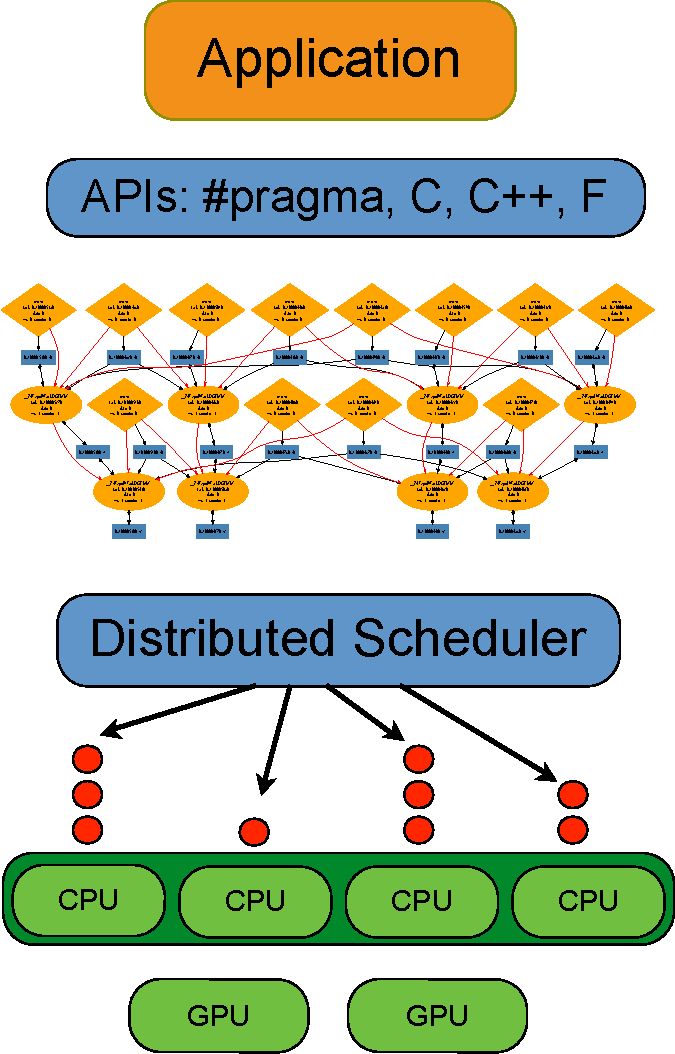
\includegraphics[width=0.7\textwidth]{kaapi-model-crop}
      \end{center}
    \end{column}
  \end{columns}
\end{frame}
%------------------------------------------------------------------------------
\begin{frame}[plain]
  \frametitle{XKaapi}
%  \vspace*{-5mm}
  \begin{figure}[ht]
  \centering
  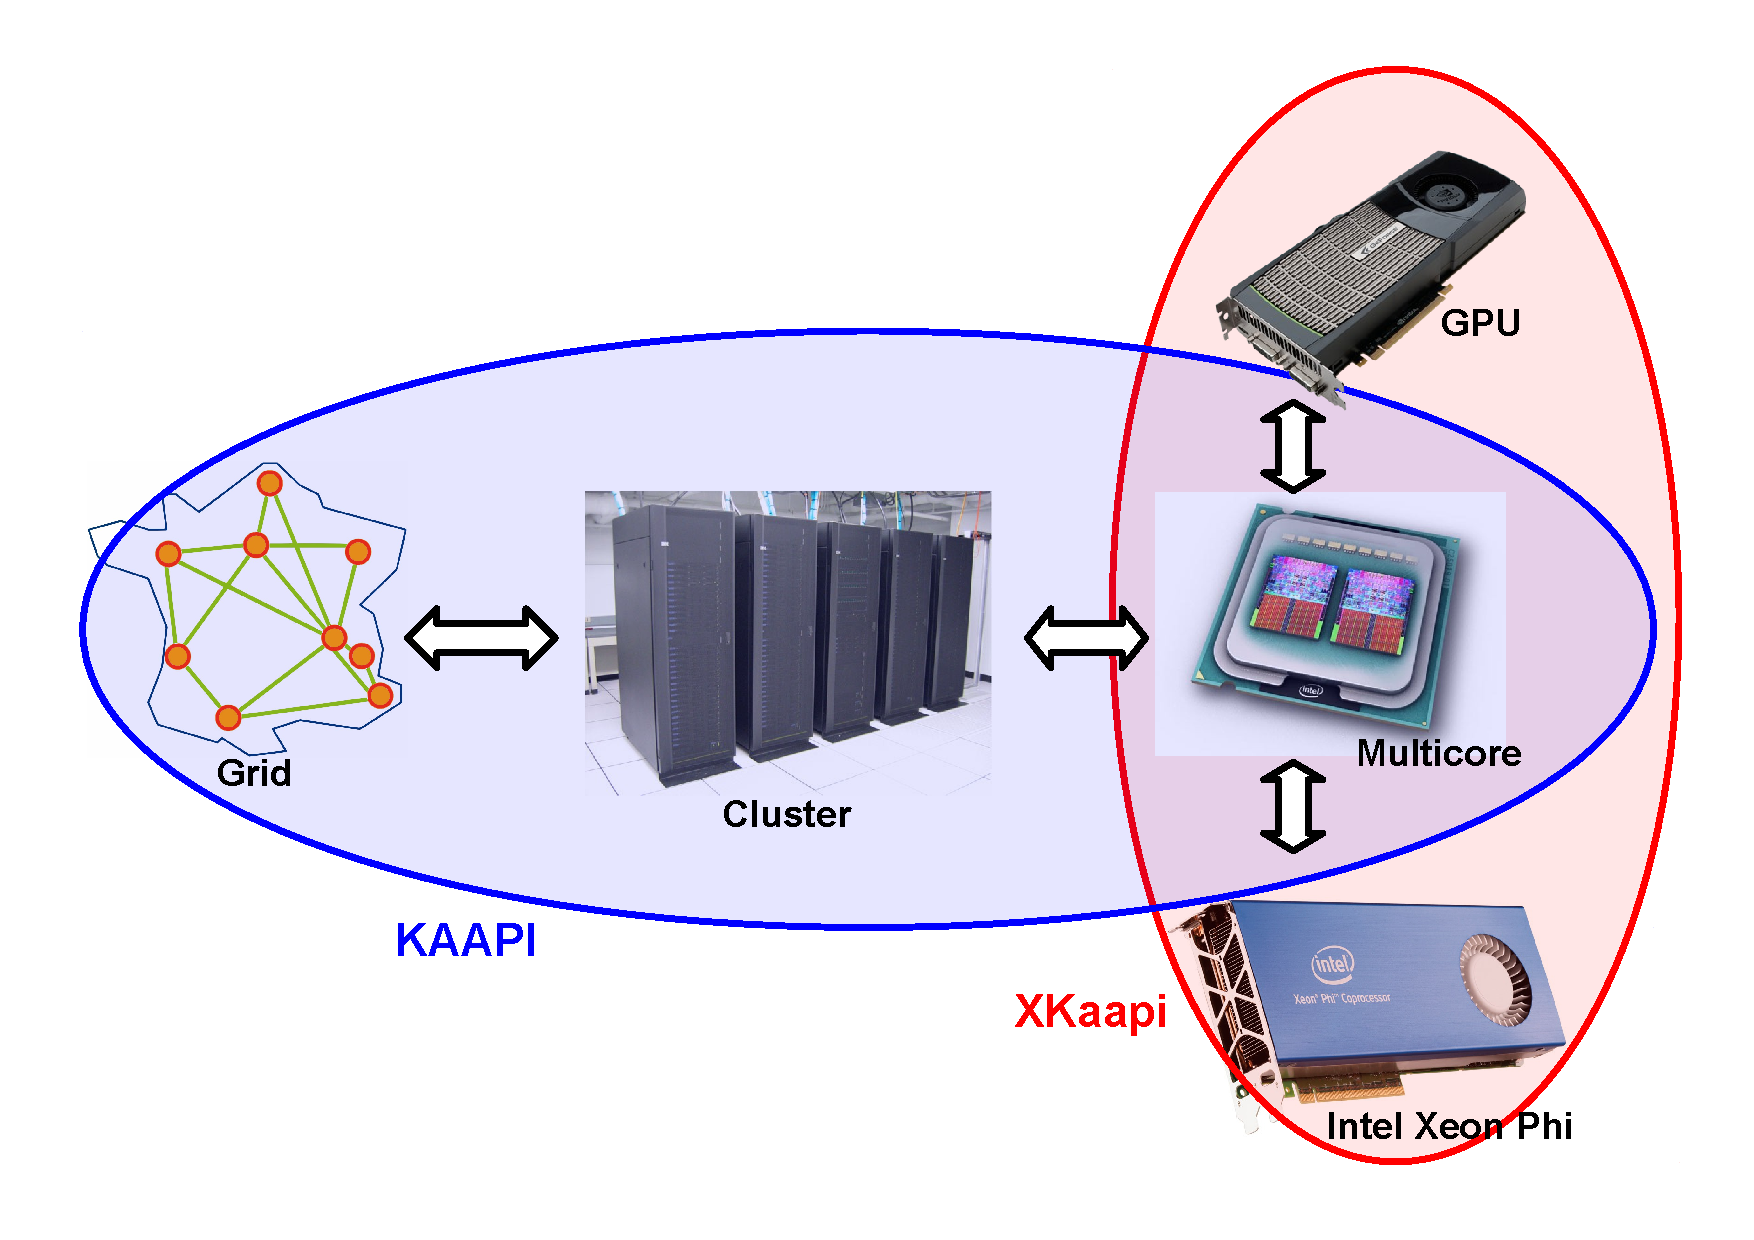
\includegraphics[width=\textwidth]{kaapi-vs-xkaapi}
  \end{figure}
\end{frame}
%------------------------------------------------------------------------------
\begin{frame}
  \frametitle{XKaapi design}
  \begin{itemize}
  \item \blue{Kernel}
    \begin{itemize}
    \item Runtime for APIs (or compiler).
    \item Work stealing internal scheduling.
    \item C language, fine grain implementation.
    \end{itemize}
  \end{itemize}

  \begin{itemize}
  \item \blue{APIs for different programming models}
    \begin{itemize}
    \item C++ API for multi-CPUs and multi-GPUs (CUDA).
    \item Two binary libraries (ABI) for OpenMP runtime
      \begin{itemize}
      \item libGOMP - GCC/OpenMP-3.1 + dependent tasks (4.0)
      \item libiomp5 - for ICC/OpenMP 3.1
      \end{itemize}
    \end{itemize}
  \end{itemize}
\end{frame}
%------------------------------------------------------------------------------
\begin{frame}[fragile]
  \frametitle{Kaapi++ API}
  \begin{itemize}
  \item Namespace \textbf{ka::}
  \end{itemize}
  %
  \begin{block}{Three main concepts}
    \begin{enumerate}
    \item {\bf Task signature} - declares parameters and their data access mode.
      \begin{itemize}
      \item Read (\verb+R+), Write (\verb+W+), Read Write (\verb+RW+),
	Cumulative Write (\verb+CW+).
      \end{itemize}
    \item {\bf Task implementation} - one implementation by architecture.
      \begin{itemize}
      \item Ex: CPU implementation, GPU implementation.
      \end{itemize}
    \item {\bf Shared data} - a data is shared between 2 tasks \textbf{iff}
      they have the same memory address in effective parameters.
    \end{enumerate}
  \end{block}
\end{frame}
%------------------------------------------------------------------------------
% \begin{frame}[fragile]
%   \frametitle{Kaapi++ API}
% \begin{block}{C++ function signature}
% \begin{lstlisting}
% void F( 
%     double n, 
%     double* result
% );
% \end{lstlisting}
% \end{block}
% %
% \pause
% %
% \begin{block}{\kaapixx task signature}
% \begin{lstlisting}
% struct TaskF: public ka::Task<2>::Signature<
%     double,       /* input parameter */
%     ka::W<double> /* output parameter */
% > {}; 
% \end{lstlisting}
% \end{block}
% \end{frame}
% %------------------------------------------------------------------------------
% \begin{frame}[fragile]
%   \frametitle{Kaapi++ API}
% \begin{block}{C++ function definition}
% \begin{lstlisting}
% void F ( 
%     double n, 
%     double* result
% ){
%     *result = n*n+1;
% }
% \end{lstlisting}
% \end{block}
% %
% \pause
% %
% \begin{block}{\kaapixx task body specialization}
% \begin{lstlisting}
% template<> struct TaskBodyCPU<TaskF> {
%     void operator() (
% 	double n,   
% 	ka::pointer_w<double> result
%     ){
% 	*result = n*n+1;
%     }
% };
% \end{lstlisting}
% \end{block}
% \end{frame}
% %------------------------------------------------------------------------------
\begin{frame}[fragile]
  \frametitle{Initialization}
%\hspace*{-4mm}
\begin{minipage}[t]{\textwidth}
%\vspace*{-6mm}
\begin{block}{}
\begin{lstlisting}
int main(int argc, char** argv) {
  try {
    /* Join the initial group of computation */
    ka::Community com = ka::System::join_community( argc, argv );
    
    /* Start computation by forking the main task */
    ka::SpawnMain<doit>()(argc, argv); 
    
    /* Leave the community */
    com.leave();

    /* */
    ka::System::terminate();
  }
  catch (const std::exception& E) {
    ka::logfile() << "Catch exception: " << E.what() << std::endl;
  }
  catch (...) {
    ka::logfile() << "Catch unknown exception: " << std::endl;
  }
  return 0;
}
\end{lstlisting}
\end{block}
\end{minipage}
\end{frame}
%------------------------------------------------------------------------------
\begin{frame}[fragile]
  \frametitle{Task entry point}
  \begin{itemize}
  \item Task ``\textbf{doit}'' spawned by the instruction \textbf{SpawnMain}.
  \end{itemize}
  %
  \begin{block}{}
  \begin{lstlisting}
/* Main task of the program
**/
struct doit {
  void operator()( int argc, char** argv )
  {
    double n = 3.1415;

    if( argc > 1 ) n = atof( argv[1] );

    /* ... */
  }
};
  \end{lstlisting}
  \end{block}
\end{frame}
%------------------------------------------------------------------------------
%\begin{frame}[fragile]
%  \frametitle{Kaapi++ tasks}
%  \begin{itemize}
%  \item {\bf Task signature}
%    \begin{itemize}
%    \item Define the number of parameters / type / access mode.
%    \end{itemize}
%  \end{itemize}
%  \vspace*{-4mm}
%\begin{block}{}
%\begin{lstlisting}
%/* Kaapi Hello task: print an integer n */
%struct TaskHello: public ka::Task<1>::Signature<int> {};
%\end{lstlisting}
%\end{block}
%%
%\pause
%%
%  \begin{itemize}
%  \item {\bf Task implementation}
%    \begin{itemize}
%    \item Specify an architecture implementation (CPU/GPU).
%    \end{itemize}
%  \end{itemize}
%  \vspace*{-4mm}
%\begin{block}{}
%\begin{lstlisting}
%/* CPU implementation */
%template<>
%struct TaskBodyCPU<TaskHello> {
%    void operator() ( int n )
%    {
%      std::cout << "Hello world in Kaapi!, n=" << n << std::endl;
%    }
%};
%\end{lstlisting}
%\end{block}
%\end{frame}
%------------------------------------------------------------------------------
\begin{frame}[fragile]
  \frametitle{Tasks}
  \begin{itemize}
  \item {\bf Task signature}
    \begin{itemize}
    \item Define the number of parameters / type / access mode.
    \end{itemize}
  \end{itemize}
  \vspace*{-4mm}
\begin{block}{}
\begin{lstlisting}
/* Kaapi Hello task: print a string and a double n */
struct TaskHello: public ka::Task<2>::Signature<std::string, double> {};
\end{lstlisting}
\end{block}
%
\pause
%
  \begin{itemize}
  \item {\bf Task implementation}
    \begin{itemize}
    \item Specify an architecture implementation (CPU/GPU).
    \end{itemize}
  \end{itemize}
  \vspace*{-4mm}
\begin{block}{}
\begin{lstlisting}
/* CPU implementation */
template<>
struct TaskBodyCPU<TaskHello> 
{
    void operator() ( std::string msg, double n )
    {
      std::cout << "Hello world in Kaapi!, msg=" << msg << ", n=" << n << std::endl;
    }
};
\end{lstlisting}
\end{block}
%
\begin{tikzpicture}[overlay,>=stealth]
\draw<3-> [draw=red,very thick] (5.8,6.1) circle (10pt);
\draw<3-> [draw=red,very thick] (9.1,6.1) ellipse (30pt and 12pt) node(a){};
\draw<3-> [draw=red,very thick] (10.8,6.1) circle (12pt) node(c){};
%
\draw<3-> [draw=red,very thick] (5.8,2.5) circle (12pt) node(b){};
\draw<3-> [draw=red,very thick] (7.8,2.5) circle (12pt) node(d){};
%
\draw<3-> [->,very thick,draw=red] (a) to (b) {};
\draw<3-> [->,very thick,draw=red] (c) to (d) {};
\end{tikzpicture}
\end{frame}
%------------------------------------------------------------------------------
\begin{frame}[fragile]
  \frametitle{Task creation}
  \begin{itemize}
  \item Keyword \textbf{spawn}.
  \end{itemize}
  \vspace*{-2mm}
\begin{block}{}
%\begin{lstlisting}
\begin{lstlisting}
/* Main task of the program */
struct doit {
  void operator()( int argc, char** argv )
  {
    double n = 3.1415;
    if( argc > 1 ) n = atof( argv[1] );

    ka::Spawn<TaskHello>()( "toto", n );
  }
};
\end{lstlisting}
\end{block}

\pause
%
  \begin{itemize}
  \item Write all arguments (integers).
  \end{itemize}
  \vspace*{-2mm}
\begin{block}{}
\begin{lstlisting}
/* The "doit" main task */
struct doit {
    void operator()( int argc, char** argv )
    {
      for(int i=1; i < argc; i++)
          ka::Spawn<TaskHello>()( std::string(argv[1]) );
    }
};
\end{lstlisting}
\end{block}
\end{frame}
%------------------------------------------------------------------------------
\begin{frame}[fragile]
  \frametitle{Execution order}
  \begin{itemize}
  \item Task creation is a non-blocking operation.
  \item the task (\blue{function call}) is pushed into a stack and the control flow
    continues without waiting for the termination. 
  \end{itemize}
  \vspace*{-2mm}
  \pause
\begin{block}{}
\begin{lstlisting}
/* The "doit" main task */
template<> struct doit {
    void operator()( int argc, char** argv )
    {
        int a;
        int* b;

        ka::Spawn<TaskThatRead_or_Write_Data>()( &a, &b );
    }
};
\end{lstlisting}
\end{block}
  \pause
  \begin{itemize}
  \item After the \blue{ka::Spawn}, task execution is not guarantee.
  \end{itemize}
\end{frame}
%------------------------------------------------------------------------------
\begin{frame}
  \frametitle{Execution order}
  \begin{itemize}
  \item Some guarantees:
    \begin{itemize}
    \item A task begins its execution when all its inputs are \red{produced}
      (\emph{data flow constraints}).
    \item  The parallel execution always produces the same result
      as the sequential execution.
    \item At the end, all created tasks have been executed. 
    \end{itemize}
  \item Notion of \blue{reference order} between tasks.
    \begin{itemize}
    \item Used to define execution order between any two tasks.
    \item Based on the Kaapi/XKaapi semantic (defined in Athapascan [1998]).
    \end{itemize}
  \end{itemize}
\end{frame}
%------------------------------------------------------------------------------
\begin{frame}[fragile]
  \frametitle{Execution order}
\begin{block}{Simple Hello world}
\begin{lstlisting}
/* The "doit" main task */
template<>
struct doit {
    void operator()( int argc, char** argv )
    {
      ka::Spawn<TaskHello>()( atoi(argv[1]) );
    }
};
\end{lstlisting}
\end{block}
%
\pause
%
\begin{block}{Possible outputs (two or mode cores)}
\begin{lstlisting}[language=]
> ./helloworld 1 2 
Hello World in Kaapi!, n=1
Hello World in Kaapi!, n=2

> ./helloworld 1 2 
Hello World in Kaapi!, n=2
Hello World in Kaapi!, n=1
\end{lstlisting}
\end{block}
\end{frame}
%------------------------------------------------------------------------------
\begin{frame}[fragile]
  \frametitle{How to enforce execution order}
  \begin{exampleblock}{Cilk's synchronization style}
    \begin{itemize}
    \item \verb+ka::Sync()+
    \item Force execution of all spawned tasks in the current task.
    \end{itemize}
  \end{exampleblock}
  %
  \pause
%  %
%  \begin{block}{Data flow constraint}
%    \begin{itemize}
%    \item \verb+ka::Sync( <pointer> )+
%    \item Wait until the pointed value is produced.
%    \end{itemize}
%  \end{block}
%  %
%  \pause
  %
  \begin{exampleblock}{Add dependencies between tasks}
    \begin{itemize}
    \item Describe \alert{access mode} of each task parameter.
    \end{itemize}
  \end{exampleblock}
\end{frame}
%------------------------------------------------------------------------------
\begin{frame}[fragile]
  \frametitle{Execution order}
\begin{block}{Simple Hello world (2 tasks)}
\begin{lstlisting}
/* The "doit" main task */
template<>
struct doit {
    void operator()( int argc, char** argv )
    {
      ka::Spawn<TaskHello>()( atoi(argv[1]) );
      ka::Sync();
      ka::Spawn<TaskHello>()( atoi(argv[1]) );
    }
};
\end{lstlisting}
\end{block}
%
\pause
%
\begin{block}{Possible outputs (two or mode cores)}
\begin{lstlisting}[language=]
> ./helloworld 1 2 
Hello World in Kaapi!, n=1
Hello World in Kaapi!, n=2

> ./helloworld 1 2 
Hello World in Kaapi!, n=1
Hello World in Kaapi!, n=2
\end{lstlisting}
\end{block}
%
\begin{tikzpicture}[overlay,>=stealth]
%\draw[<-] (1,1) .. (3,3) node[above] {\bf Cria};
\draw<3-> [<-,line width=2pt] (2.9,5.3) -- (9,5.3) node[shape=rectangle,fill=red!30] {Enforce order};
\draw<3-> [<-,line width=2pt] (4.6,2.2) -- (8,2.2) node[shape=rectangle,fill=green!30] {Always the same order};
%\node<3-> [shape=rectangle,fill=blue!20,below of=t1] {Recomendado quando $N = O(nthreads)$.};
\end{tikzpicture}
%
\end{frame}
%------------------------------------------------------------------------------
\begin{frame}[fragile]
  \frametitle{How to enforce execution order}
  \begin{itemize}
  \item Paramater rules: \blue{effective parameters}
    are mapped to \blue{formal parameters}.
  \end{itemize}
  %
  \pause
  %
  \begin{block}{By value}
    \begin{itemize}
    \item a copy is made into the task.
    \end{itemize}
  \end{block}
  %
  \pause
  %
  \begin{block}{By reference}
    \begin{itemize}
    \item No copy.
    \item But tasks must declare its acesses to shared data. 
    \item \textbf{read}: read access, the task can read the value.
    \item \textbf{write}: write access, a reader will see the written value.
    \item \textbf{read write}: exclusive access, one task has access to data.
    \item \textbf{cumulative write}:  several write will participate to produce the final
      value.
    \end{itemize}
  \end{block}
\end{frame}
%------------------------------------------------------------------------------
\begin{frame}[fragile]
  \frametitle{Task signature}
%\vspace*{-4mm}
%  \begin{itemize}
%  \item Número de parâmetros fixo em tempo de compilação.
%  \end{itemize}
%\hspace*{-4mm}
\begin{minipage}[t]{\textwidth}
\begin{block}{}
\begin{lstlisting}
/* Kaapi Hello task: print an integer n */
struct TaskFibo: public ka::Task<2>::Signature<ka::W<int>, int> {};
\end{lstlisting}
\end{block}
\end{minipage}
%
  \begin{itemize}
  \item<2-> \blue{Access mode}
    \begin{itemize}
    \item \verb+ka::W<T>+ - write.
    \item \verb+ka::R<T>+ - read.
    \item \verb+ka::RW<T>+ - read and write.
    \item \verb+ka::CW<T>+ - cumulative write with reduction.
    \end{itemize}
  \item<3-> \blue{Formal parameter}
    \begin{itemize}
    \item \verb+ka::pointer_w<T>+
    \item \verb+ka::pointer_r<T>+
    \item \verb+ka::pointer_rw<T>+
    \item \verb+ka::pointer_cw<T>+
    \end{itemize}
  \end{itemize}
\end{frame}
%------------------------------------------------------------------------------
\begin{frame}[fragile]
  \frametitle{Task implementation}
%  \vspace*{-4mm}
\begin{block}{}
\begin{lstlisting}
/* Kaapi Hello task: print an integer n */
struct TaskFibo: public ka::Task<2>::Signature<ka::W<long>, long> {};
\end{lstlisting}
\end{block}
%
\onslide<2->
%
\begin{block}{}
\begin{lstlisting}
/* CPU implementation */
template<>
struct TaskBodyCPU<TaskFibo> {
    void operator() ( ka::pointer_w<long> ptr, long n )
    {
        if (n < 2){ 
          *ptr = n; 
          return;
	} else {
          ka::auto_pointer<long> ptr1 = new long;
          ka::auto_pointer<long> ptr2 = new long;

          ka::Spawn<TaskFibo>() ( ptr1, n-1 );
          ka::Spawn<TaskFibo>() ( ptr2, n-2 );

          ka::Spawn<TaskSum>() ( ptr, ptr1, ptr2 );      
	}
    }
};
\end{lstlisting}
\end{block}
%
\begin{tikzpicture}[overlay,>=stealth]
\draw<3-> [draw=red,very thick] (5.7,7.8) circle (10pt);
\draw<3-> [draw=red,very thick] (9.3,7.8) circle (12pt) node(a){};
\draw<3-> [draw=red,very thick] (10.5,7.8) circle (12pt) node(c){};
%
\draw<3-> [draw=red,very thick] (6.2,5.8) circle (12pt) node(b){};
\draw<3-> [draw=red,very thick] (8.1,5.8) circle (12pt) node(d){};
%
\draw<3-> [->,very thick,draw=red] (a) to (b) {};
\draw<3-> [->,very thick,draw=red] (c) to (d) {};
\end{tikzpicture}
%
\end{frame}
%------------------------------------------------------------------------------
\begin{frame}
  \frametitle{Dependency}
  \begin{itemize}
  \item Task must describe its data access modes in effective parameters.
    \begin{itemize}
    \item Task signature.
    \item No side effect!
    \end{itemize}
  \item At runtime: execution $=$ sequence of tasks.
  \end{itemize}
  \begin{exampleblock}{XKaapi always respect the following dependencies:}
    \begin{itemize}
    \item A reader will see the value written by the last task in the reference order:
      \begin{itemize}
      \item W $\rightarrow$ R, {CW}* $\rightarrow$ R, ou RW $\rightarrow$ R: {\bf Read After Write}.
      \end{itemize}
    \item Other false dependencies (\textbf{Write after Read}) may be resolved by 
      \blue{additional data copies}.
      \begin{itemize}
      \item Runtime decision.
      \end{itemize}
    \end{itemize}
  \end{exampleblock}
\end{frame}
%------------------------------------------------------------------------------
\begin{frame}
  \frametitle{Dependency cost}
  \begin{block}{Dependency analysis is required to execute two tasks in parallel}
    \begin{itemize}
    \item Tasks with dependencies are executed following the \blue{reference order}.
      \begin{itemize}
      \item ``A reader will see the value written by the last writer''.
      \end{itemize}
    \item Tasks without dependencies may execute in parallel.
      \begin{itemize}
      \item The \blue{runtime} decides when and where 2 concurrent tasks will execute in parallel. 
      \end{itemize}
    \end{itemize}
  \end{block}
  %
  \pause
  %
  \begin{alertblock}{Work stealing scheduler}
    \begin{itemize}
    \item Execution following the reference order of execution.
      \begin{itemize}
      \item Only  \blue{dequeue}, no dependency analysis.
      \end{itemize}
    \item Dependencies are only computed during \blue{steal operation}.
    \end{itemize}
  \end{alertblock}
\end{frame}
%------------------------------------------------------------------------------
\begin{frame}[fragile]
  \frametitle{What is really shared ?}
  \begin{itemize}
  \item Two tasks sahred a common data \textbf{IFF} they access 
    the same data in memory.
  \item In the current implementation, it is a \red{limitation}.
    \begin{itemize}
    \item {\bf same data == same pointer}.
    \end{itemize}
  \end{itemize}
  %
\begin{block}{}
\begin{lstlisting}
ka::pointer<T> a;
ka::pointer<T> b = a + 100;
ka::Spawn<TaskRW1>()( a ); /* rw on a */
ka::Spawn<TaskRW2>()( b ); /* rw on b */
\end{lstlisting}
\end{block}
%
  \begin{alertblock}{No memory region (yet)}
  {\bf TaskRW1} and {\bf TaskRW2} are independent, even if 
  ``a'' and ``b'' overlap.
  \end{alertblock}
\end{frame}
%------------------------------------------------------------------------------
\begin{frame}[fragile]
  \frametitle{Example}
\begin{block}{}
\begin{lstlisting}[basicstyle=\scriptsize\ttfamily]
struct TaskFibo: public ka::Task<2>::Signature<ka::W<long>, long> {};

struct TaskDelete: public ka::Task<1>::Signature<ka::RW<long> > {};

struct TaskPrint: public ka::Task<1>::Signature<ka::R<long> > {};

int main( void ) {
  ka::pointer<long> res = new long;
  ka::Spawn<TaskFibo>()( res, n );


  ka::Spawn<TaskPrint>()( res );


  ka::Spawn<TaskDelete>()( res ); // free memory 
}
\end{lstlisting}
\end{block}
%
\begin{itemize}
\item The runtime automatically detects dependencies between tasks.
\item \blue{Write after Read} dependencies may be solved by copy.
\end{itemize}
%
\begin{tikzpicture}[overlay,>=stealth]
\draw<2-> [->,line width=2pt,red,bend left] (3.9, 4.1) .. controls(4.1,3.7) .. (3.9, 3.3) 
    node[above right=4pt,] {W $\rightarrow$ R (true) dependency};
\draw<2-> [->,line width=2pt,red,bend left] (3.9, 3.2) .. controls(4.1,2.8) .. (3.9, 2.4) 
    node[above right=4pt,] {R $\rightarrow$ RW (false) dependency};
\end{tikzpicture}
\end{frame}
%------------------------------------------------------------------------------
% \begin{frame}[fragile]
%   \frametitle{API Kaapi++}
% \begin{block}{C++ function calls}
% \begin{lstlisting}
% F(n, &result);
% Print(&result);
% \end{lstlisting}
% \end{block}
% %
% \pause
% %
% \begin{block}{\kaapixx task creation}
% \begin{lstlisting}
% ka::Spawn<TaskF>()(n, &result);
% ka::Spawn<TaskPrint>()(&result);
% ka::Sync();
% \end{lstlisting}
% \end{block}
% \end{frame}
%------------------------------------------------------------------------------
\begin{frame}[fragile]
  \frametitle{XKaapi source}
  \begin{itemize}
  \item \url{http://kaapi.gforge.inria.fr}
    \begin{itemize}
    \item Last version: \textbf{2.2}
    \end{itemize}
  \item Git: ligforge
    \begin{itemize}
    \item url $\rightarrow$ \url{ssh://git.ligforge.imag.fr/git/kaapi/xkaapi.git}
    \end{itemize}
  \item Git branches
    \begin{itemize}
    \item \verb+origin/master+: the oficial master branch.
    \item \verb+origin/<username>/<branch name>+: an user branch. 
    \end{itemize}
  \item Mailing list: \url{kaapi-leaders@lists.gforge.inria.fr}
    \begin{itemize}
    \item \url{http://lists.gforge.inria.fr/cgi-bin/mailman/listinfo/kaapi-leaders}
    \end{itemize}
  \end{itemize}
\end{frame}
%------------------------------------------------------------------------------
\begin{frame}[fragile]
  \frametitle{Installation}
  \begin{itemize}
  \item Requirement:
    \begin{itemize}
    \item GCC $>=$ 4.4 or Clang $>=$ 3.4
    \end{itemize}

  \item automake / autotools / etc...
    \begin{itemize}
    \item \verb+../xkaapi/configure --help+
    \item \verb+../xkaapi/configure --prefix=<prefixdir>+
    \item Usefull options:
      \begin{itemize}
      \item \verb+--enable-mode=release+ for performance.
      \item \verb+--enable-mode=debug+ for more assertions in the user level.
      \item \verb+--with-perfcounter+ for performance counter and tracing.
      \end{itemize}
    \end{itemize}
 
    \item Compiling \& installing
      \begin{itemize}
      \item make; make install
      \end{itemize}
  \end{itemize}
\end{frame}
%------------------------------------------------------------------------------
\begin{frame}[fragile]
  \frametitle{Running}
  \begin{itemize}
  \item \verb|KAAPI_CPUCOUNT=1 ./fibo_kaapi++ 30+|
      \begin{block}{}
      \begin{lstlisting}[language=]
Fibo(30)=832040
Time: 4.326541e-01
      \end{lstlisting}
      \end{block}
  \item \verb|KAAPI_CPUCOUNT=2 ./fibo_kaapi++ 30|
      \begin{block}{}
      \begin{lstlisting}[language=]
Fibo(30)=832040
Time: 2.143562e-01
      \end{lstlisting}
      \end{block}
  \item \verb|KAAPI_CPUSET=0:4,6 ./fibo_kaapi++ 30|
    \begin{itemize}
    \item Use cores 0,1,2,3,4 and 6 of the machine.
    \end{itemize}
  \end{itemize}
\end{frame}
%------------------------------------------------------------------------------
%------------------------------------------------------------------------------
% - %\subsection*{Installation de XKaapi}
% - \begin{frame}
% -   \frametitle{XKaapi installation}
% - 
% -   Installation (\p{make install}) into the directory \p{prefix}.
% - 
% -   Classic structure:
% -   \begin{itemize}
% -   \item \p{<prefix>/include} : header files
% -   \item \p{<prefix>/lib} : libraries
% -   \item \p{<prefix>/lib/pkgconfig} : \p{pkg-config} files
% -     to retrieve compilation flags 
% -   \item \p{<prefix>/share/doc/xkaapi} :  documentation
% -   \item \p{<prefix>/share/doc/xkaapi/examples} : examples in many APIs
% -     with a Makefile to compile
% -   \end{itemize}
% - \end{frame}
% - %------------------------------------------------------------------------------
% - %\subsection*{Installation alternative par paquets binaires}
% - %------------------------------------------------------------------------------
% - \begin{frame}
% -   \frametitle{Alternative installation}
% -   For Debian (Ubuntu ?), binary installation from packages.
% -   \begin{alertblock}{Attention}
% -     \begin{itemize}
% -     \item Packages are not in the official repositories.
% -     \item Compilation for the ``unstable'' distribution, see
% -       ``experimental'' (for CUDA 5)
% -     \end{itemize}
% -   \end{alertblock}
% - %
% -   \begin{enumerate}
% -   \item Add sources to \p{/etc/apt/sources.list}
% -     \begin{code}
% -       \hspace{-1cm}\footnotesize deb http://people.debian.org/~vdanjean/debian unstable main
% -     \end{code}
% -   \item \p{apt-get update}
% -   \item \p{apt-get install vdanjean-keyring}
% -   \item \p{apt-get update}
% -   \item \p{apt-get install libkaapi++-dev}
% -   \item \p{apt-get install -t experimental nvidia-cuda-toolkit libcupti-dev}
% -   \end{enumerate}
% - 
% - \end{frame}
% - %------------------------------------------------------------------------------
% - %\subsection{Compilation de programmes}
% - %------------------------------------------------------------------------------
% - \begin{frame}
% -   \frametitle{Compiling a XKaapi program}
% -   To compile a XKaapi program:
% -   \begin{enumerate}
% -   \item If the prefix is not standard (\p{/usr} ou \p{/usr/local}),
% -     configure \alert{\p{PKG\_CONFIG\_PATH}} :
% -     \begin{code}
% -       \footnotesize export PKG\_CONFIG\_PATH=<kaapi
% -       prefix>/lib/pkgconfig
% -     \end{code}
% - 
% -   \item Compile and link with \alert{\p{pkg-config}} :
% -     \begin{code}
% -       g++ -o mytest `pkg-config -{}-cflags kaapi++` $\backslash$ \\
% -       ~~~~`pkg-config -{}-libs kaapi++` mytest.cpp
% -     \end{code}
% -   \end{enumerate}
% - \end{frame}
% - %------------------------------------------------------------------------------
% - %\subsection{Exécution de programmes}
% - \begin{frame}
% -   \frametitle{Execute a XKaapi program}
% -   \begin{enumerate}
% -   \item If the prefix is not standard (\p{/usr} ou \p{/usr/local}),
% -     configure \alert{\p{LD\_LIBRARY\_PATH}} :
% -     \begin{code}
% -       \footnotesize export LD\_LIBRARY\_PATH=<kaapi prefix>/lib
% -     \end{code}
% - 
% -   \item Program execution:
% -     \begin{code}
% -       ./mytest
% -     \end{code}
% -   \end{enumerate}
% -   XKaapi can be ``configured'' with environment variables:
% -   \begin{code}\small
% -   \alert{KAAPI\_CPUCOUNT=1} ./fibo\_kaapi++ 30\\
% -   \structure{Fibo(30)=832040 Time: 4.326541e-01}\\
% -   \alert{KAAPI\_CPUCOUNT=2} ./fibo\_kaapi++ 30\\
% -   \structure{Fibo(30)=832040 Time: 2.143562e-01}\\
% -   \alert{KAAPI\_CPUSET=0:4,6} ./fibo\_kaapi++ 30\\
% -   \# use cores 0,1,2,3,4 and 6 of the machine
% -   \end{code}
% - 
% - \end{frame}
% - %------------------------------------------------------------------------------
% - %\subsection*{OpenMP et XKaapi}
% - \begin{frame}
% -   \frametitle{Execute an OpenMP program with XKaapi}
% -   \begin{enumerate}
% -   \item Compile the OpenMP program with \p{gcc} (with no XKaapi).
% -   \item Execute the program with the wrapper \p{libkomp-run}
% -     (installed into \p{<kaapi prefix>/bin}) :
% -     \begin{code}
% -       libkomp-run ./program-OpenMP
% -     \end{code}
% -   \item Compare execution against GCC runtime:
% -     \begin{code}
% -       ./program-OpenMP
% -     \end{code}
% -   \end{enumerate}
% - \end{frame}
% - %------------------------------------------------------------------------------
%%%%%%%%%%%%%%%%%%%%%%%%%%%%%%%%%%%%%%%%%%%%%%%%%%%%%%%%%%%%%%%%%%%%%%%%%%%%%%%
\subsection{OpenMP 4}
%------------------------------------------------------------------------------
%\begin{frame}
%  \frametitle{OpenMP 4}
%\end{frame}
%------------------------------------------------------------------------------
\begin{frame}[fragile]
  \frametitle{OpenMP 4}
  \begin{itemize}
  \item OpenMP 4.0 includes data dependency between tasks (\texttt{task}).
  \pause
  \item Directive \texttt{depend}
    \begin{itemize}
    \item \texttt{in} -- read.
    \item \texttt{out} -- write.
    \item \texttt{inout} -- read and write.
    \end{itemize}
  \pause
  \item Recursive synchronization by \texttt{taskgroup} construct.
    \begin{itemize}
    \item Synchronize a structured block.
    \item \texttt{taskgroup} waits for \alert{descendant tasks}.
    \item \texttt{taskwait} \alert{wait on the completion of child tasks}.
    \end{itemize}
  \end{itemize}
%
\pause
%
\begin{block}{Data flow dependency}
\begin{lstlisting}
#pragma omp taskgroup
{
  #pragma omp task depend(in:data) \
    depend(out:result)
  foo(data, result);
}
\end{lstlisting}
\end{block}
%
\end{frame}
%------------------------------------------------------------------------------
\begin{frame}[fragile]
  \frametitle{OpenMP 4}
\begin{block}{Fibonacci with OpenMP \texttt{depend}}
\begin{lstlisting}
int fib( int n ) {
  int x, y;
  if( n < 2 ) return n;
  #pragma omp taskgroup
  {
    #pragma omp task shared(x) depend(in:n) \
        depend(out:x)
    x = fib( n - 1);
    #pragma omp task shared(y) depend(in:n) \
      depend(out:y)
    y = fib( n - 2);
  }
  return x + y;
}
\end{lstlisting}
\end{block}
\end{frame}
%------------------------------------------------------------------------------
\begin{frame}[fragile]
  \frametitle{OpenMP 4 support}
  \begin{itemize}
  \item Clang with Intel OpenMP runtime library.
    \begin{itemize}
    \item \url{http://clang-omp.github.io/}
    \item \url{http://openmp.llvm.org/}
    \end{itemize}
  \item GCC (4.9) with libgomp runtime.
    \begin{itemize}
    \item \url{https://gcc.gnu.org/wiki/openmp}
    \end{itemize}
  \end{itemize}
\end{frame}
%------------------------------------------------------------------------------
%------------------------------------------------------------------------------
